\section{Time to frequency and frequency to time}
\subsection{Toolbox: Spectrum}
Most of the \texttt{make\_spectrum} function is already given. All that is missing is generation of the frequency vector.
The output of \texttt{fft} returns the spectrum values starting with the DC element, followed by the positive frequency values
and then the negative frequency values. As the resolution in the frequency domain is \(\frac{1}{T}\), where \(T\) is the period of 
the signal to be transformed, the following code can be used to generate a frequency vector compatible with the output of \texttt{fft}.

\begin{lstlisting}[
style=Matlab-editor,
basicstyle=\ttfamily\footnotesize,
numbers=none]
% Frequency vector
T = length(signal)/fs; %signal sample time
delta_f = 1/T; %frequency resolution
freq = [0:delta_f:fs/2-delta_f,-fs/2:delta_f:0-delta_f]; %fft spits out DC,positive frequencies and then negative freqs
\end{lstlisting}

\begin{figure}
	\center
	\includegraphics{./picture/3-1-1.eps}
	\caption{Fourier transform of a 1kHz sine wave with amplitude 1, sampled at 10kHz over 1 second}
	\label{fig:1.1}
\end{figure}

The result of applying the \texttt{make\_spectrum} function to a sinusoid with amplitude 1 and a frequency of 1kHz, sampled at 10kHz over
a period of 1 second, can be seen in figure~\ref{fig:1.1}.
